\documentclass[12pt]{article}

\usepackage{sbc-template}

\usepackage{graphicx,url}
\usepackage{mathptmx}
\usepackage{graphicx}
\usepackage{times}
\usepackage{enumitem}
\usepackage[]{algorithm2e}
\usepackage[table,xcdraw]{xcolor}
\usepackage{pdfpages}
\usepackage{booktabs}

%\usepackage[brazil]{babel}   
\usepackage[latin1]{inputenc} 


\title{Discrete Fourier Transform for Dummies}

\author{Alex Frasson and Tiago Augusto Engel\inst{1}}


\address{Universidade Federal de Santa Maria (UFSM)\\ 
	\email{\{afrasson,tengel\}@inf.ufsm.br}
}

\begin{document} 
\maketitle

\section{Introduction}

\section{The Real DFT}

nesse link explica 

http://www.analog.com/media/en/technical-documentation/dsp-book/dsp\_book\_Ch31.pdf

While historically most theorists engineers find easier to work with the complex form, the Fourier transform can be calculated using real numbers as well. 

\begin{equation}
ReX(k)=\frac{2}{N} \sum_{n=0}^{N-1}f(n) \cos(2\pi kn/N)
\end{equation}
\begin{equation}
ImX(k)=\frac{-2}{N} \sum_{n=0}^{N-1}f(n) \sin(2\pi kn/N)
\end{equation}

The N sample time domain signal $f(n)$ is decomposed into a set of N/2+1 cosine, and N/2+1 sine waves, with frequencies given by the index $k$. The amplitudes of the cosine waves are contained in $ReX(k)$, while the amplitudes of the sine waves are contained in $ImX(n)$. These  equations operate by correlating the respective cosine or sine wave with the time domain signal.  In spite of using the names: real part and imaginary part, there are no complex  numbers in these equations\cite{Analog2016}.


\section{1D DFT Definition}
\begin{equation}
F(u)=\sum_{x=0}^{M-1}f(x) e^{-j 2\pi u x / N}
\end{equation}
where $u = 0,1,2,\dots, M-1$

\begin{equation}
f(x)=\frac{1}{M}\sum_{u=0}^{M-1}F(u) e^{j 2\pi u x / N}
\end{equation}
where $x = 0,1,2,\dots, M-1$

%\subsection{Implementation}

\begin{figure}[!htbp]
	\begin{center}
		\leavevmode
		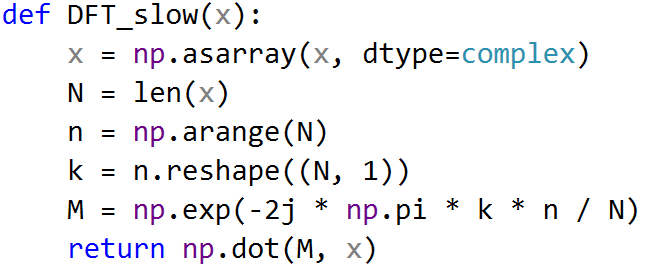
\includegraphics[width=8cm]{images/dft.png}
		\caption{1D DFT python implementation.}
	\end{center}
\end{figure}

\section{2D DFT Definition}
The 2D transform can be obtained by calculating the 1D of the rows of the image, following by the same function applied to the columns.

\begin{equation}
F(k,l)=\frac{1}{MN}\sum_{m=0}^{M-1}\sum_{n=0}^{N-1} f(m,n) e^{-j 2\pi (\frac{km}{M} + \frac{ln}{N})}
\end{equation}
where $m = 0,1,2,\dots, M-1$ and $n = 0,1,2,\dots, N-1$

\begin{equation}
f(m,n)=\sum_{k=0}^{M-1}\sum_{l=0}^{N-1} F(k,l) e^{j 2\pi (\frac{km}{M} + \frac{ln}{N})}
\end{equation}
where $k = 0,1,2,\dots, M-1$ and $l = 0,1,2,\dots, N-1$

\begin{figure}[!htbp]
	\begin{center}
		\leavevmode
		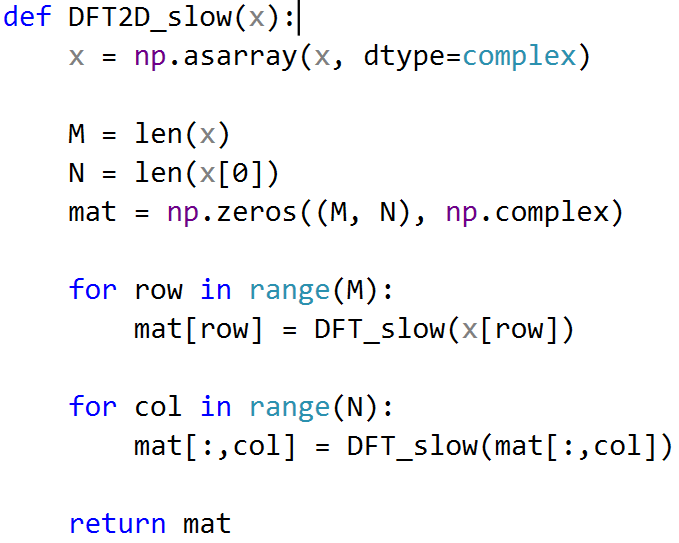
\includegraphics[width=8cm]{images/dft2d.png}
		\caption{2D DFT python implementation.}
	\end{center}
\end{figure}


\subsection{The spectrum}
The norm of the amplitude, or Fourier spectrum is defined as the image corresponding to the length of each complex number. Indeed, we can calculate the length of the complex number as:
\begin{equation}
	|F(u,v)|= (R^2(u,v) + I^2(u,v))^{1/2}
\end{equation}

The spectrum can be visualized by calculating the aforementioned formula. However, in order to properly visualize it, we need to translate the top-left corner to the center of the image. This can be done by applying the transform from -M/2 to M/2 or simply multiplying the input image by $(-1)^{x+y}$ \cite{Gonzalez2008}.

\begin{figure}[!htbp]
	\begin{center}
		\leavevmode
		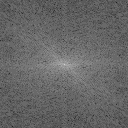
\includegraphics[scale=1]{images/spectrum.png}
		\caption{Fourier spectrum example.}
	\end{center}
\end{figure}

Finally, as the frequency components u and v are zero at the origin, it is often referred to as DC component. This component corresponds to the highest magnitude in the image, and is the average of all other samples.

\subsection{Phase angle}
The phase angle is defined as:
\begin{equation}
	\phi(u,v) = \arctan(\frac{I(u,v)}{R(u,v)})
\end{equation}

Even though phase information is not used as much as the spectrum information, there are specific applications where it is useful. If we construct synthetic images made from the amplitude information of one image and the phase information of another, it is the image corresponding to the phase data that we perceive, if somewhat degraded. We can see this effect in the following figure.

\begin{figure}[!htbp]
	\begin{center}
		\leavevmode
		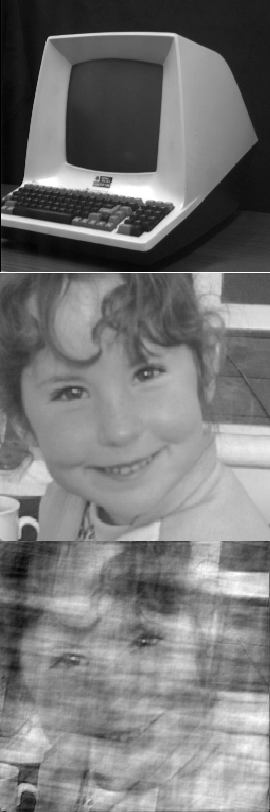
\includegraphics[scale=1]{images/phase.png}
		\caption{Fourier spectrum example.}
		\label{fig:rasterData}
	\end{center}
\end{figure}

\bibliographystyle{sbc}
\bibliography{references}

\end{document}
